\chapter{Introduction}

\label{ch1_INTRO}

%Replace \lipsum with text.
% You may have as many sections as you please. This is just for reference.





\section{Introduction}
Human activity recognition is an area of interest in the field of large scale surveillance.
A highly accurate and precise system would obviate the need for human attention
at each of the surveillance video output all the time. The system can recognize the
actions being performed by the human in the video and can decide for itself if the actions are abnormal;
in which case, it may raise an alarm for human attention.

This project tries to improve the existing activity recognition system
by adding domain knowledge and support for uncertainty to it.

\begin{comment}
% You may add figures in the following manner.
\begin{figure}[here]
\begin{center}	
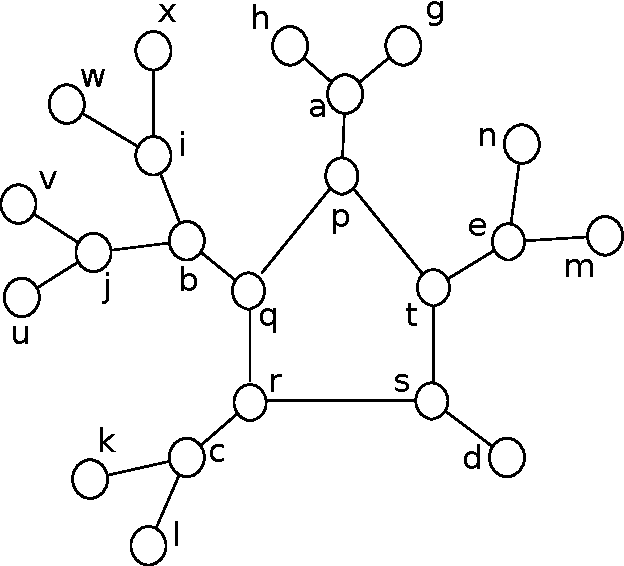
\includegraphics[scale=0.4]{pent} 
\caption{Pentagon $pqrst$}
\label{fig:pent}
\end{center}
\end{figure}
\end{comment}




\section{Related Work}
In \cite{Realistic}, authors have come up with a method to annotate video clips 
from Hollywood movies using their text scripts.
Authors present a method for classification using local space-time features, space-time pyramids 
and multi-channel non-linear SVM. The method of classification is similar to that explained in chapter \ref{ch2_STIP}. 
In \cite{actionsInContext}, authors have also added scene information to the classification.

In \cite{improving}, authors have used object information present in the video clip. 
The correlation between activity and object has been found using analysis of large amount of text. 
Note that this correlation is not found directly via video but via text.
Thus it has the limitation that only the correlations appearing in the text can be captured.
Finally an integrated classifier is formed which combines classification based on methods from chapter \ref{ch2_STIP} 
and probability of activity deduced from object information.








\section{Motivation}
Existing activity recognition systems do not take advantage of underlying domain.
Domain may have significant influence over the activity types, the objects appearing
in the activity etc. For example, presence of a dining table improves the chances
of activity eating as compared to driving. Or if, the video is occluded partially,
but objects like bottle and chair are visible, then also, chances of activity eating
are more as compared other activities. This relationship between objects and activities
can be captured by First Order Logic (FOL).

But merely using FOL is not sufficient. In its basic form, FOL uses hard constraints.
To explain this with example, consider a rule
\begin{equation}
	\label{MLNRule}
	\forall clip ~ HasObject( clip, bottle ) \implies HasActivity( clip, eating )
\end{equation}

In real world scenario, it is perfectly possible that a video clip contains a bottle,
but the activity might be different than eating. 
The rule gets violated in this scenario as it is universally quantified over all the clips. 
Rule may also get violated in case of noisy training data. 
Thus, using hard constraints is neither practical nor robust for real world video clips. 

Solution to this is to attach weights with rules like \eqref{MLNRule} with weights being proportional to the real world relevance.
This idea can be captured using Markov Logic Networks (MLNs).








\section{Problem Statement}
As evident from previous section, existing methods use video and object features. They do not capture domain information, i.e. correlation between object and activity. 
This project captures the correlation as well as makes the system more robust towards noisy training data.
Problem statement of this project is to improve the existing human activity recognition systems
by incorporating domain knowledge using Markov Logic Networks (MLN).








\section{Data set Description}
Data set used in this project is standard Hollywood2 (actions) data set from \cite{actionsInContext}. 
It has 823 labeled training video clips and 884 labeled testing video clips. 
There are 12 activity classes : AnswerPhone, DriveCar, Eat, FightPerson,
 GetOutCar, HandShake, HugPerson, Kiss, Run, SitDown, SitUp, StandUp.
 Each clip is 10 to 30 seconds long.


\section{Approach}
\begin{itemize}
	\item A support vector machine model is learnt using the video features of training data set. 
	\item Presence of objects in video clips is found along with the confidence of detection using object detector. 
	\item MLN model is learnt to capture the correlation between activity and object.
	\item Learnt MLN model is used to classify test video clips.
\end{itemize}

Figure \ref{fig:approach} explains the approach
\begin{figure}[H]
\begin{center}	
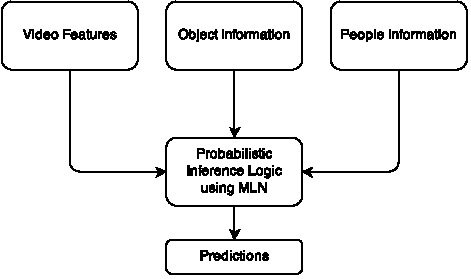
\includegraphics[trim=80 150 80 90,clip,scale=0.4]{approach} 
\caption{Approach}
\label{fig:approach}
\end{center}
\end{figure}


\section{Thesis Outline}
Chapter \ref{ch2_STIP} explains video classification using only video features. It explains how to extract and use the video features. 
Chapter \ref{ch3_OBJ} describes object detection in detail. 
Chapter \ref{ch4_MLN} describes the theory of Markov Logic Networks. 
Chapter \ref{ch5_RESULTS} shows the result comparisons.
Finally thesis concludes with chapter \ref{ch6_CONCLUSION} which notes conclusion and future work.

\begin{comment}
\begin{table}
\centering
\begin{tabular}{| c | c |}
\hline
{\bf item 1} & {\bf item 2} \\ \hline
%
abcde & 5 \\ \hline
%
pqrst & 4 \\ \hline
\end{tabular}
\caption{A sample table}
\label{table:1}
\end{table}
\end{comment}


